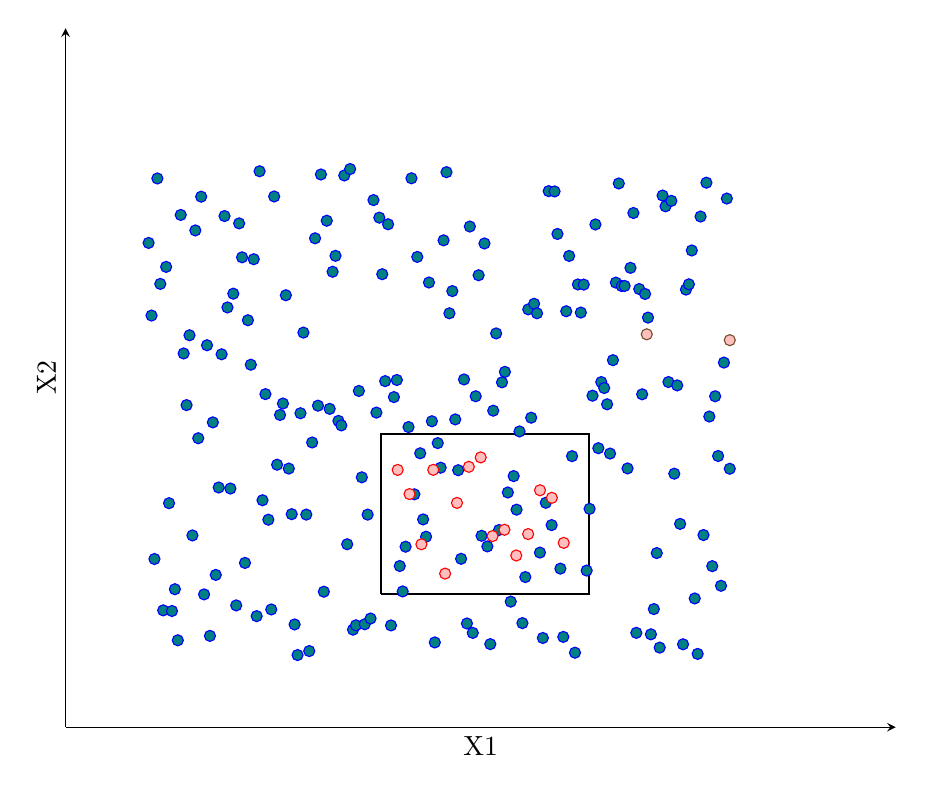
\begin{tikzpicture}
  \begin{axis}[
        width=\linewidth,
        xmin=0,xmax=10,ymin=0,ymax=100, 
        xlabel=X1,
        ylabel=X2,
        ticks=none,
        axis x line=bottom,axis y line=left
        ]
       \addplot+[y filter/.expression={y+10},only marks,mark=*, mark options = {fill=teal},samples=200,domain=1:8] {70*rnd};
       \addplot+[y filter/.expression={y+20},only marks,mark=*,mark options={fill=pink},samples=15,domain=4:6] {20*rnd};
      \addplot+[y filter/.expression={y+50},only marks,mark=*,mark options={fill=pink},samples=2,domain=7:8] {20*rnd};
       \draw[thick] (3.8, 19) -- (6.3,19) -- (6.3,42) -- (3.8, 42) -- (3.8, 19);
  \end{axis}
\end{tikzpicture}